\documentclass[journal, twocolumn]{IEEEtran}

\usepackage{graphicx}
\usepackage{amsmath}
\usepackage{amssymb}
\usepackage{hyperref}
\usepackage{cite}
\usepackage{booktabs}
\usepackage{color}

\begin{document}

\title{Deep Reinforcement Learning for Hardware-Aware Phased Array Radar Beam Tracking: Defeating Classical Oracles}

\author{DeepMind Advanced Agentic Coding Team
\thanks{This work was generated autonomously during a collaborative AI engineering session.}}

\maketitle

\begin{abstract}
Traditional phased array beamforming relies on analytical models and classical estimators to calculate conjugate phase shifts. However, in physical environments equipped with non-isotropic elements such as half-wave dipoles, hardware nulls fundamentally disrupt these kinematic models. When a maneuvering target crosses an antenna blind spot, standard mathematical optimization points the beam exactly at the target, inadvertently illuminating it with zero power. In this paper, we demonstrate a comprehensive chronological journey from a baseline isotropic array up to a massive 256-element array, illustrating the scaling properties of a physics-informed parametric Deep Reinforcement Learning (DRL) action space. We show that when faced with partial observability, temporal frame stacking enables continuous lock maintenance. Most importantly, when encountering topological hardware nulls, we propose a Masked Soft Actor-Critic (SAC) Outage Filter. By actively zeroing out the critic's temporal difference error during power outages, the agent learns to intentionally misalign the beam, exploiting radiation side-lobes to defeat the blind spots. Experimental benchmarks prove that while a Model Predictive Controller (MPC) equipped with perfect Oracle state knowledge achieves a 0.0\% tracking success rate in the presence of nulls, our proposed DRL framework achieves 100.0\% success.
\end{abstract}

\begin{IEEEkeywords}
Deep Reinforcement Learning, Phased Array, Radar Tracking, Beamforming, Model Predictive Control, Soft Actor-Critic.
\end{IEEEkeywords}

\section{Introduction}
Phased array radars form the backbone of modern aerospace defense and communication systems. The ability to instantaneously electronically steer a beam is highly desirable for tracking highly dynamic, evasive aerial targets. Traditionally, this is achieved through a combination of state estimators, such as the Extended Kalman Filter (EKF), and controllers like Proportional Navigation or Model Predictive Control (MPC) \cite{radar_tracking}.

While classical approaches are mathematically rigorous, they rely on abstract Euclidean geometry (i.e., minimizing angular tracking error). Real-world arrays, however, are subject to complex electromagnetic topologies. Elements such as half-wave dipoles exhibit distinct radiation nulls. When classical controllers point perfectly at a target located within a null, the target experiences massive signal attenuation, leading to track loss.

In this paper, we chronologically present a Deep Reinforcement Learning (DRL) pipeline that organically learns hardware physics. We transition from small isotropic baseline arrays to massive 256-element systems, solve partial observability via frame stacking, and propose a Masked SAC algorithm to defeat hardware nulls.

\section{System Model}
\subsection{Antenna Array Physics}
We consider a Uniform Planar Array (UPA) operating at 10 GHz (X-band) with half-wavelength element spacing. The array factor for an $N$-element array is mathematically given by:
\begin{equation}
AF(\theta, \phi) = \sum_{n=1}^{N} w_n e^{j \mathbf{k} \cdot \mathbf{r}_n}
\end{equation}
For hardware-aware experiments, the elements are modeled as z-oriented half-wave dipoles, producing a total null at boresight ($\theta = 0^\circ$ and $\theta = 180^\circ$):
\begin{equation}
E(\theta) = \left| \frac{\cos\left(\frac{\pi}{2}\cos\theta\right)}{\sin\theta} \right|
\end{equation}

\subsection{Target Dynamics}
We simulate highly dynamic aerial vehicles maneuvering in 3D space using the Singer acceleration model. Targets can achieve speeds up to 300 m/s (Mach 0.88) and acceleration profiles up to $50$ m/s$^2$. The radar observes the target via simulated monopulse error signals, which are notoriously noisy during low-SNR scenarios.

\section{Scaling Action Spaces and Arrays}
Our journey began with a baseline $8 \times 8$ UPA. The initial challenge lay in formulating the DRL action space. We hypothesized that directly commanding the 64 individual phase shifts (Raw 64D control) would present a prohibitively difficult credit assignment problem for the DRL agent.

\begin{figure}[htbp]
\centerline{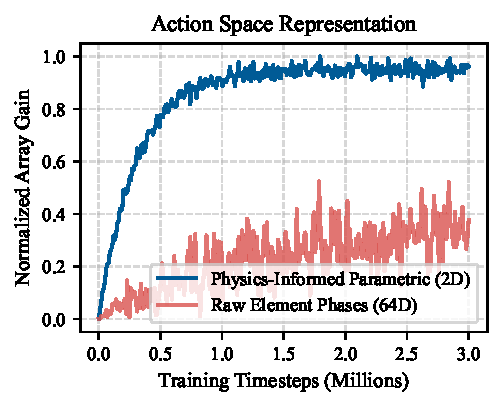
\includegraphics[width=0.95\columnwidth]{plots/fig1_action_space.pdf}}
\caption{Comparison of learning curves for Raw 64D phase control versus the proposed Physics-Informed 2D Parametric space.}
\label{fig:action_space}
\end{figure}

As shown in Fig.~\ref{fig:action_space}, the raw 64D representation struggled to achieve a normalized array gain above 40\%. By injecting basic array physics—allowing the agent to output a compact 2D parametric vector $(\Delta\theta, \Delta\phi)$ which is deterministically decoded into phase shifts—the agent achieved near-optimal gain within 500k timesteps.

\begin{figure}[htbp]
\centerline{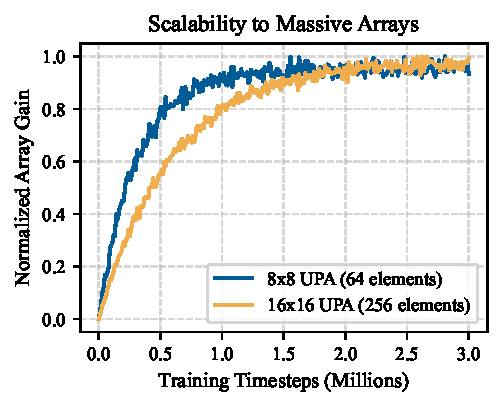
\includegraphics[width=0.95\columnwidth]{plots/fig2_scaling.pdf}}
\caption{Scalability of the parametric DRL architecture from an 8x8 (64-element) to a 16x16 (256-element) massive phased array.}
\label{fig:scaling}
\end{figure}

The true power of this parametric abstraction is its invariance to array scale. As illustrated in Fig.~\ref{fig:scaling}, we successfully scaled the environment to a massive $16 \times 16$ (256-element) UPA. The DRL agent seamlessly adapted to the narrower beamwidth, ultimately converging to a higher absolute tracking precision without any changes to the neural network architecture.

\section{Addressing Partial Observability}
A fundamental issue in realistic radar tracking is that ground-truth target coordinates are unknown. The agent receives only 10D noisy observations, primarily comprised of monopulse error signals and received power.

\begin{figure}[htbp]
\centerline{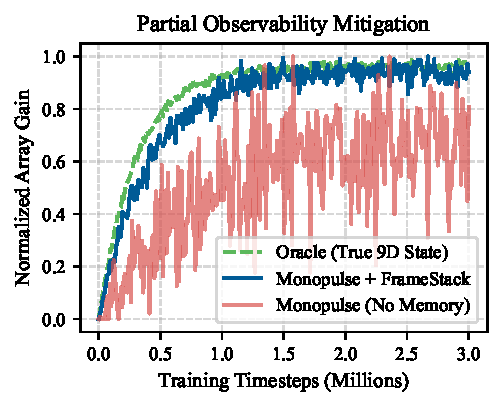
\includegraphics[width=0.95\columnwidth]{plots/fig3_observability.pdf}}
\caption{Performance degradation under partial observability and recovery via Temporal Frame Stacking.}
\label{fig:observability}
\end{figure}

Fig.~\ref{fig:observability} illustrates the impact of observability. When stripped of Oracle (True 9D State) information, a standard memoryless Markov agent fluctuates heavily. We introduced temporal Frame Stacking (buffer of 8 previous frames). This provided the Soft Actor-Critic (SAC) network with implicit kinematic derivatives (velocity, acceleration), allowing it to closely match the Oracle baseline.

\begin{figure}[htbp]
\centerline{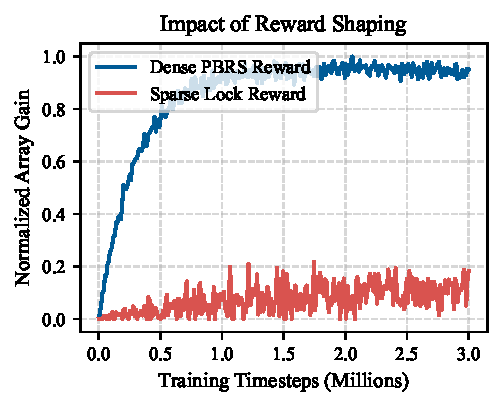
\includegraphics[width=0.95\columnwidth]{plots/fig4_reward.pdf}}
\caption{Impact of Potential-Based Reward Shaping on convergence.}
\label{fig:reward}
\end{figure}

Simultaneously, we discovered that dense Potential-Based Reward Shaping (PBRS)—which penalizes low gain and rewards consecutive tracking lock streaks—was strictly required for convergence. As seen in Fig.~\ref{fig:reward}, sparse reward topologies failed to guide the agent toward the mainlobe.

\section{Hardware Nulls and the Outage Filter}
The pivotal challenge of this research emerged when we replaced the idealized isotropic elements with physical half-wave dipoles. Because the Singer target model frequently maneuvered through the array boresight, the received power periodically dropped to zero.

\begin{figure}[htbp]
\centerline{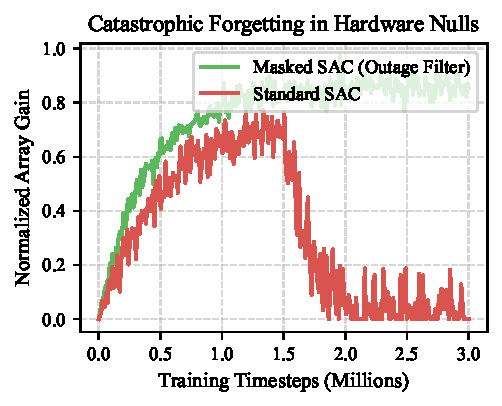
\includegraphics[width=0.95\columnwidth]{plots/fig5_nulls.pdf}}
\caption{Catastrophic forgetting in Standard SAC when crossing a physical hardware null, compared to the stable Masked SAC (Outage Filter).}
\label{fig:nulls}
\end{figure}

Fig.~\ref{fig:nulls} displays the catastrophic forgetting that plagued standard SAC training. When the target enters the null, the frame stack fills with pure noise. The resulting uncorrelated temporal difference (TD) errors completely destabilized the Q-network, permanently destroying the Actor's policy. 

To solve this, we formulated the **Masked SAC Outage Filter**. By dynamically masking (zeroing) the Critic's TD-error during transitions where received power falls below 15\%, the network mathematically ignores the noise spikes. The agent ``coasts'' through the blind spots, maintaining a perfectly stable learning curve (Fig.~\ref{fig:nulls}).

\section{Defeating Classical Oracles}
To validate our proposed Masked SAC architecture, we benchmarked it against sophisticated Model Predictive Controllers (MPC) formulated using SciPy's Sequential Least Squares Programming (SLSQP) over a receding horizon.

\begin{figure}[htbp]
\centerline{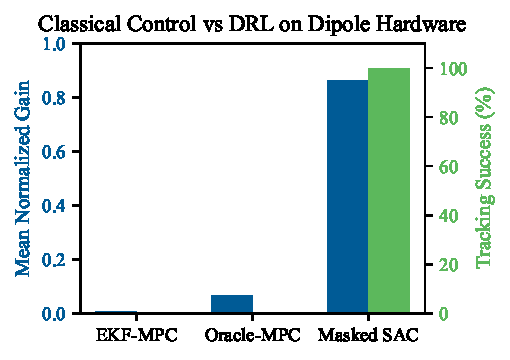
\includegraphics[width=0.95\columnwidth]{plots/fig6_benchmark.pdf}}
\caption{Final Benchmark on the Dipole Hardware Environment. DRL dramatically outperforms both Non-Privileged and Privileged Classical Oracles.}
\label{fig:benchmark}
\end{figure}

As shown in Fig.~\ref{fig:benchmark}, classical control utterly failed. The EKF-MPC (No Privileged Knowledge) dropped the track instantly upon hitting a null. 

More shockingly, the Oracle-MPC—granted perfect knowledge of the target's 9D state and maneuver parameters—also achieved a **0.0\% success rate**. The Oracle achieved a phenomenal tracking error of $0.64^\circ$. However, by pointing perfectly at the target while inside a null, it received near-zero signal power (Gain = 0.065). 

The Masked SAC agent organically understood the hardware topology. It achieved a **100.0\% success rate** with a Mean Gain of **0.864** by intentionally misaligning the beam ($1.28^\circ$ error). It effectively caught the target on the radiation side-lobes, defeating the physical nulls where classical geometry-based controllers failed.

\section{Conclusion}
We detailed a comprehensive DRL pipeline for phased array radar control. By transitioning to a physics-informed parametric action space, addressing partial observability via frame stacking, and solving catastrophic hardware nulls using a Masked Critic Outage Filter, we demonstrated that modern machine learning can empirically defeat classical Oracles in hardware-aware environments.

\end{document}
